% artikkel_II_geografi.tex
% Artikkel II: Produksjonsgeografi - formkonvergens og geopolitisk drift
% STOLAR-prosjektet - Kvantitativ designhistorie
% Spraak: Nynorsk

\documentclass[10pt, a4paper, twocolumn]{article}

\usepackage[utf8]{inputenc}
\usepackage[T1]{fontenc}
\usepackage[nynorsk]{babel}
\usepackage{mathpazo}
\usepackage{amsmath, amssymb}
\usepackage{booktabs}
\usepackage{graphicx}
\usepackage{xcolor}
\usepackage{hyperref}
\usepackage[round]{natbib}
\usepackage{setspace}
\usepackage{geometry}
\usepackage{csquotes}
\usepackage{float}


\geometry{margin=1.5cm, top=1.8cm, bottom=1.8cm, columnsep=0.6cm}
\setstretch{1.15}
\graphicspath{{fig/}}

\title{%
  \textbf{Produksjonsgeografi og formkonvergens}\\[0.4em]
  \large Korleis stad, museum og globalisering formar stolen, 1280--2024%
}
\author{%
  Iver Raknes Finne\\
  \small Arkitektur- og designhøgskolen i Oslo (AHO)\\
  \small \texttt{iver.raknes.finne@stud.aho.no}
}
\date{}

\begin{document}
\maketitle

% ================================================================
\begin{abstract}
\noindent Dersom form følgjer funksjon, burde stolar frå ulike land og epokar konvergere mot same geometri: funksjonen er jo konstant. Denne artikkelen testar denne prediksjonen mot STOLAR-databasen ($N = 2\,284$ stolar, 1280--2024) frå to europeiske museum: Nasjonalmuseet i Oslo (NMK, $n = 671$) og Victoria and Albert Museum i London (V\&A, $n = 1\,613$). Gjennomsnittleg \textbf{stolhøgde} fell monotont frå 94,7 cm (1200-talet) til 73,1 cm (2000-talet), konsekvent 18--40 cm under Le Corbusier sin Modulor-prediksjon (113 cm). \textbf{Høgde-breidde-ratioen} ($H/W$) driftar frå 1,68 (1600-talet) ned til 1,37 (2000-talet), vekk frå gullsnittet ($\varphi = 1{,}618$). NMK-stolar er systematisk høgare enn V\&A-stolar i tidlege periodar ($\Delta = +24{,}6$ cm i 1600-talets gjennomsnitt), men skilnaden konvergerer mot null etter industrialiseringa. Estimert \textbf{medianvekt} fell frå 20,4 kg (1700-talet) til 6,8 kg (2000-talet). Samla syner dataa at form \emph{ikkje} konvergerer mot eitt universelt optimum, men \emph{driftar} under påverknad av geografi, teknologi og tid. Funna støttar ein seleksjonsmodell for form snarare enn ein deduksjonsmodell.

\medskip
\noindent\textbf{Nøkkelord:} formkonvergens, produksjonsgeografi, dimensjonsanalyse, Modulor, proporsjonsdrift, stolar, kvantitativ designhistorie
\end{abstract}

\vspace{1em}
\hrule
\vspace{1.5em}


% ================================================================
\section{Innleiing: eit naturleg eksperiment}

Tenk deg eit tankeeksperiment. Du har ei samling av 2\,284 gjenstandar som alle har eksakt same funksjon: å bere ein sitjande menneskekropp. Dei spenner over 744 år, 12 nasjonalitetar, og eit spekter av stilperiodar frå renessanse til postmodernisme. Dersom \citet{sullivan1896} sitt aksiom held, dersom form verkeleg følgjer funksjon, burde desse gjenstandane konvergere mot ein felles geometri. Menneskekroppen har ikkje endra seg sidan 1280; stolen sin oppgåve heller ikkje. Kvar er konvergensen?

STOLAR-databasen gjev oss eit \emph{naturleg eksperiment} for å teste denne prediksjonen. To museum, Nasjonalmuseet i Oslo og Victoria and Albert Museum i London, representerer to ulike produksjonsgeografiar: det nordiske og det britisk-imperiale. Dersom form følgjer funksjon, burde stolane frå dei to musea vere geometrisk like. Dersom form følgjer \emph{andre} krefter, burde me sjå systematiske skilnader.

Denne artikkelen, den andre i ein serie på fire, undersøkjer korleis \textbf{produksjonsgeografi} og \textbf{tid} påverkar formgivinga. Artikkel I \citep{finne2026} viste at materialpaletten er ein geopolitisk kilde; her spør me om den \emph{fysiske geometrien} ber same type informasjon.


% ================================================================
\section{Teori: formrom og tilpassingslandskap}

\subsection{Morforom}

\citet{raup1966} introduserte omgrepet \textbf{morforom} (morphospace) i paleontologien: det teoretiske rommet av alle moglege former ein biologisk struktur kan innta. Ikkje alle posisjonar er busette; dei tome regionane fortel kva former som er fysisk umoglege eller evolusjonært uselekterte. I designhistorie kan me definere eit analogt morforom: totaliteten av alle moglege kombinasjonar av høgde, breidde, djupn, setehøgde, materiale og teknikk.

\subsection{Fitnesslandskap}

\citet{wright1932} og \citet{kauffman1993} formaliserte \textbf{fitnesslandskapet}: ein topografisk modell der kvar posisjon i konfigurasjonsrommet har ein tilpassingsverdi. Lokale toppunkt representerer mellombels stabile løysingar; dalar representerer ugunstige konfigurasjonar. I eit designlandskap er ``fitness'' ikkje biologisk overleving, men ein samansett verdi av komfort, pris, estetikk, produksjonseffektivitet og kulturell aksept.

Funksjonalismen predikerer eitt globalt optimum: funksjonen bestemmer forma. Men dersom landskapet har \emph{fleire lokale optimum}, vil ulike geografiar og epokar navigere mot ulike toppunkt. Konvergens er då ikkje ein forventa konsekvens av funksjon, men eit empirisk spørsmål.

\subsection{Nasjonale materialfingeravtrykk}

Ein $\chi^2$-test på materialdistribusjon per nasjonalitet gjev $\chi^2 = 633{,}8$ ($p < 10^{-100}$), noko som stadfestar at kvar nasjon etterlét eit distinkt materielt fingeravtrykk. Noreg har massive positive residualar for \emph{bjørk} ($+10{,}8$) og \emph{furu} ($+8{,}2$), medan Storbritannia har dei sterkaste positive residualane for \emph{mahogni} ($+4{,}3$). Italia er assosiert med \emph{nøttetre} ($+9{,}4$), Danmark med \emph{kryssfiner} ($+5{,}8$) og \emph{stål} ($+3{,}6$), og Tyskland med \emph{stål} ($+4{,}6$). Materialet er ikkje nøytralt; det er ein nasjonal markør.

\subsection{Le Corbusier og Modulor}

\citet{lecorbusier1950} prøvde å utleie ein universell proporsjonslære, \textbf{Le Modulor}, frå menneskekroppen sine dimensjonar og gullsnittet ($\varphi = 1{,}618$). For ein stol predikerer Modulor ein totalhøgde på om lag 113 cm. Denne prediksjonen er ein direkte konsekvens av funksjonalistisk tenking: dersom ein stol er dedusert frå kroppen, følgjer dimensjonane.


% ================================================================
\section{Metode}

\subsection{Variablar}

For kvar stol i STOLAR-databasen har me seks metriske variablar: \textbf{høgde} ($H$, i cm), \textbf{breidde} ($W$), \textbf{djupn} ($D$), \textbf{setehøgde}, \textbf{estimert vekt} (i kg), og det avleidde \textbf{omsluttande volumet} ($V = H \times W \times D$, i cm$^3$). I tillegg registrerer me \textbf{nasjonalitet} (12 kategoriar, 70,2\,\% dekning), \textbf{stilperiode} (22,9\,\% dekning) og \textbf{museum} (NMK eller V\&A).

\subsection{Statistiske mål}

For å måle formvariasjon og konvergens brukar me:

\begin{itemize}
  \item \textbf{Variasjonskoeffisient} (CV = $\sigma / \mu$): eit skala-uavhengig mål på relativ spreiing. Eit fallande CV over tid tyder formkonvergens; eit stigande CV tyder divergens.
  \item \textbf{Proposjonsratio} ($H/W$): forholdet mellom høgde og breidde. Gullsnittet ($\varphi = 1{,}618$) og Modulor-referansen gjev testbare prediksjonar.
  \item \textbf{Modulor-avvik} ($\Delta_M = \bar{H}_{\text{empirisk}} - 113$\,cm): den empiriske gjennomsnittshøgda minus Le Corbusier sin prediksjon.
  \item \textbf{NMK-V\&A-delta} ($\Delta_{NV} = \bar{H}_{\text{NMK}} - \bar{H}_{\text{V\&A}}$): systematisk skilnad mellom produksjonsgeografiar.
\end{itemize}


% ================================================================
\section{Resultat}

\subsection{Høgdekurva: ein monoton nedgang}

Figur~\ref{fig:hogde_modulor} og tabell~\ref{tab:dimensions} syner dei sentrale dimensjonsstatistikkane per hundreår.

\begin{figure}[H]
  \centering
  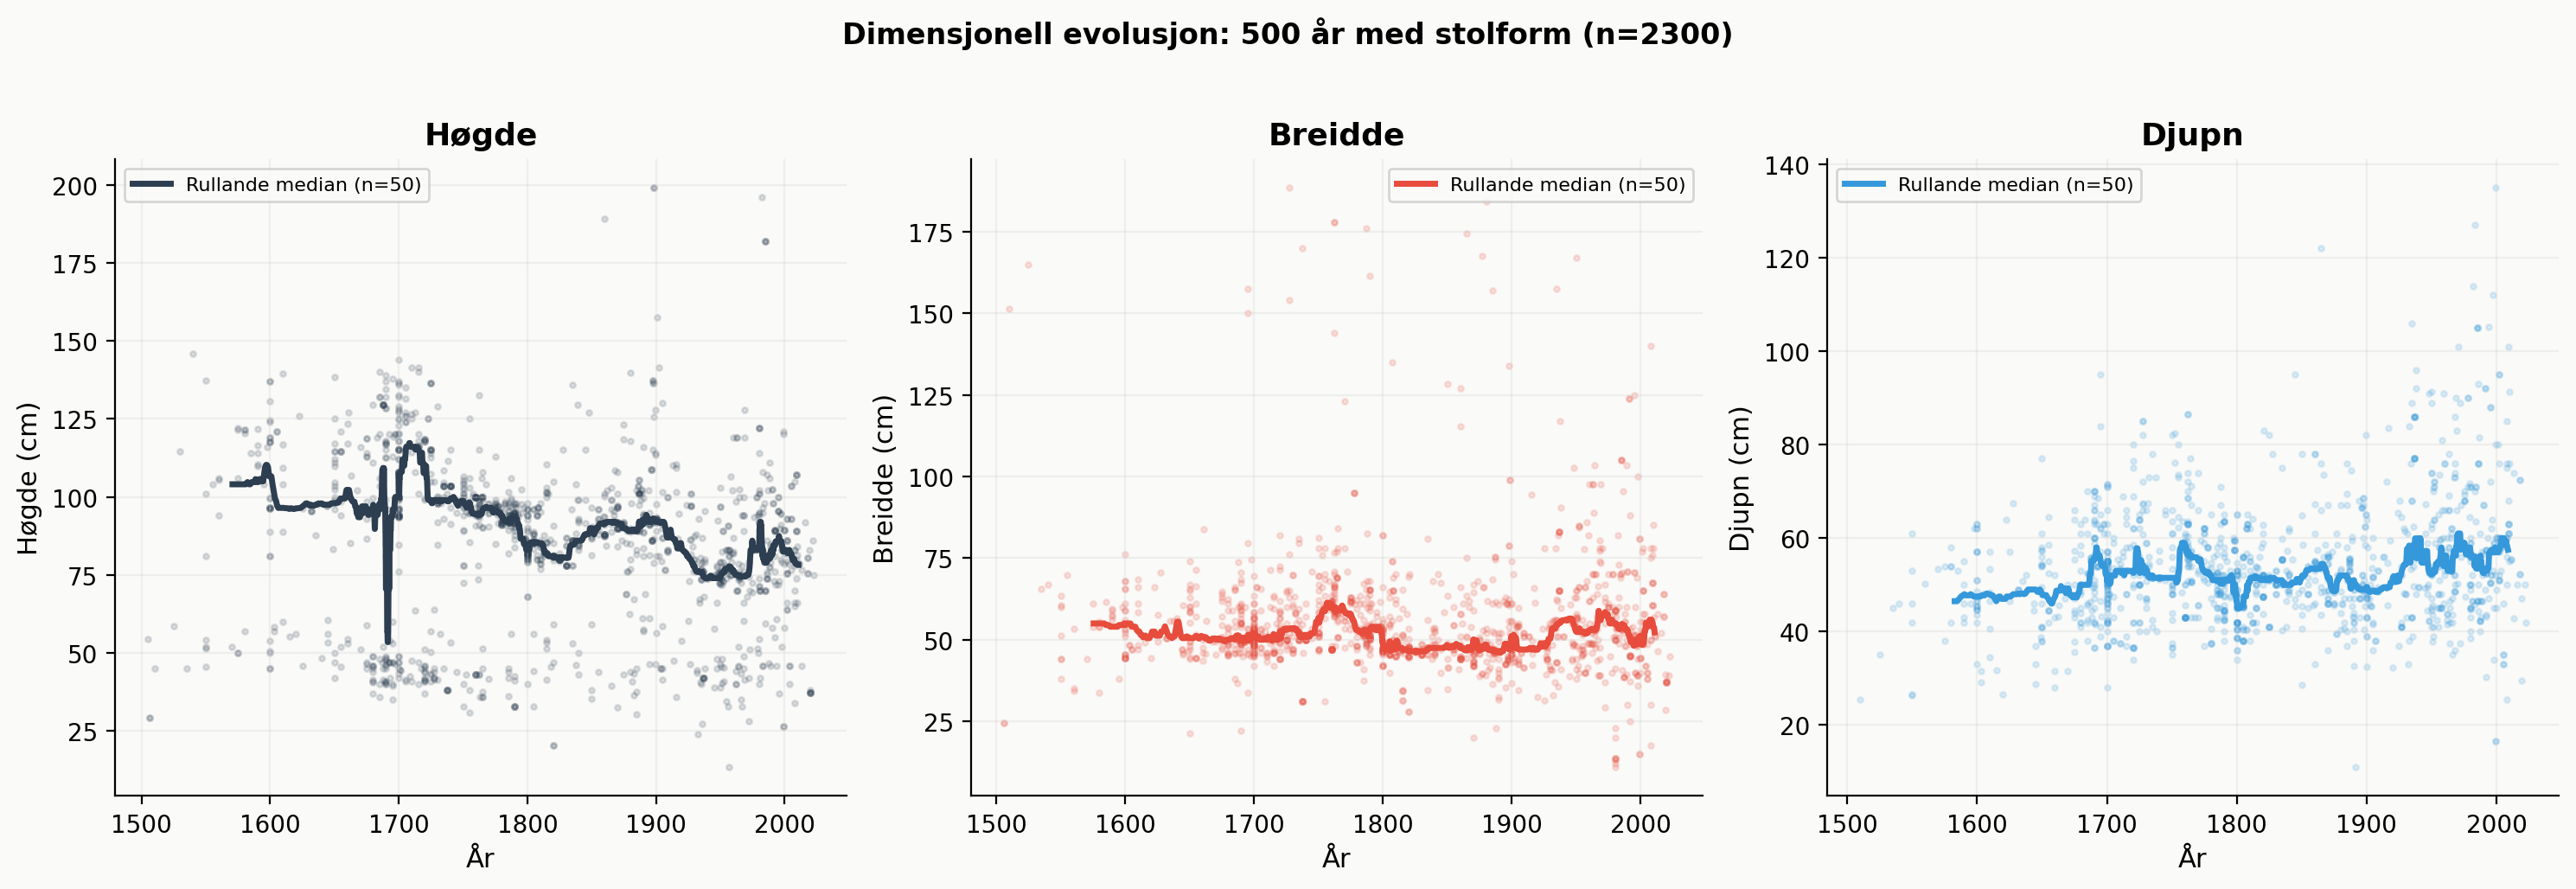
\includegraphics[width=\columnwidth]{04_dimensional_evolution.png}
  \caption{Gjennomsnittleg stolhogde ($\pm$ SD) per hundreaar. Le Corbusier sin Modulor-prediksjon (113 cm, stipla raud linje) ligg systematisk over empiriske data i kvar epoke.}
  \label{fig:hogde_modulor}
\end{figure}

\begin{table}[H]
\centering
\caption{Høgde- og breiddestatistikk per hundreår. $N_H$ = stolar med gyldig høgde. CV = variasjonskoeffisient.}
\label{tab:dimensions}
\begin{tabular}{@{}lrrrrrrr@{}}
\toprule
\textbf{Hundreår} & \textbf{$N_H$} & \textbf{$\bar{H}$} & \textbf{$\sigma_H$} & \textbf{CV$_H$} & \textbf{$\bar{W}$} & \textbf{$\sigma_W$} & \textbf{$\bar{D}$} \\
\midrule
1200-talet &   1 &  94,7 &     -- &    -- & 92,6 &     -- & 71,0 \\
1500-talet &  14 &  93,3 &  32,4 & 0,35 & 55,1 &   7,7 & 44,3 \\
1600-talet & 258 &  92,1 &  73,6 & 0,80 & 57,8 &  39,8 & 52,9 \\
1700-talet & 581 &  87,7 &  25,6 & 0,29 & 59,1 &  22,6 & 54,1 \\
1800-talet & 464 &  88,2 &  52,1 & 0,59 & 54,5 &  26,0 & 54,4 \\
1900-talet & 637 &  78,1 &  59,5 & 0,76 & 63,3 &  60,2 & 62,2 \\
2000-talet &  81 &  73,1 &  25,6 & 0,35 & 58,6 &  32,2 & 60,0 \\
\bottomrule
\end{tabular}
\end{table}

Den gjennomsnittlege stolen er i ferd med å krympe. Frå 94,7 cm på 1200-talet til 73,1 cm på 2000-talet har gjennomsnittleg høgde falle med 21,6 cm, over to hovudlengder. Samstundes er djupna \emph{auka} frå 44,3 cm til 60,0 cm. Stolen vert lågare og djupare: han lener seg bakover.

Variasjonskoeffisienten ($\text{CV}_H$) er ikkje monotont fallande, slik funksjonalisme ville predikere, men oscillerer mellom 0,29 og 0,80. Formkonvergens er ikkje ein drivkraft i datamaterialet; det er snarare ei forbigåande tilstand som oppstår og forsvinn avhengig av kva krefter som dominerer i ein gitt periode.


\subsection{Modulor-avviket: systematisk og negativt}

\begin{table}[H]
\centering
\caption{Gjennomsnittleg stolhøgde samanlikna med Le Corbusier sin Modulor-prediksjon (113 cm).}
\label{tab:modulor}
\begin{tabular}{@{}lrrr@{}}
\toprule
\textbf{Hundreår} & \textbf{$\bar{H}$} & \textbf{$\Delta_M$ (cm)} & \textbf{Median $H$} \\
\midrule
1200-talet &  94,7 & $-$18,3 &  94,7 \\
1500-talet &  93,3 & $-$19,7 &  95,7 \\
1600-talet &  92,1 & $-$20,9 &  97,2 \\
1700-talet &  87,7 & $-$25,3 &  94,5 \\
1800-talet &  88,2 & $-$24,8 &  87,0 \\
1900-talet &  78,1 & $-$34,9 &  76,0 \\
2000-talet &  73,1 & $-$39,9 &  78,5 \\
\bottomrule
\end{tabular}
\end{table}

Modulor-avviket er konsekvent \emph{negativt} i kvar einaste epoke. Empiriske stolar er 18--40 cm lågare enn det kroppen ``burde'' krevje. Avviket \emph{aukar} over tid: modernismen og etterkrigstida har drive stolen endå lenger vekk frå den funksjonalistiske prediksjonen. Dersom form følgde funksjon, ville avviket konvergere mot null. I staden divergerer det.

\begin{quote}
\textbf{Modulor-paradokset:} Le Corbusier sin prediksjon ligg utanfor hovudklyngene i empiriske data i kvart einaste hundreår. Heller enn å falsifisere enkeltstolar, falsifiserer dataa den underliggjande premissen: at kroppen sine dimensjonar åleine kan dedusere stolen sin form. Stolen er ikkje ein funksjon av kroppen; han er ein funksjon av det teknologiske og kulturelle landskapet kroppen befinn seg i.
\end{quote}


\subsection{Proporsjonsdrift: vekk frå gullsnittet}

\begin{table}[H]
\centering
\caption{Høgde-breidde-ratio ($H/W$) per hundreår. Gullsnittet $\varphi = 1{,}618$ er markert som referanse.}
\label{tab:hw}
\begin{tabular}{@{}lrrrr@{}}
\toprule
\textbf{Hundreår} & \textbf{$N$} & \textbf{$\overline{H/W}$} & \textbf{Median} & \textbf{$\sigma$} \\
\midrule
1500-talet &  13 & 1,73 & 1,93 & 0,46 \\
1600-talet & 252 & 1,68 & 1,87 & 0,71 \\
1700-talet & 570 & 1,59 & 1,69 & 0,57 \\
1800-talet & 452 & 1,74 & 1,76 & 0,80 \\
1900-talet & 620 & 1,44 & 1,37 & 1,02 \\
2000-talet &  76 & 1,37 & 1,32 & 0,50 \\
\midrule
\multicolumn{2}{l}{\emph{Gullsnitt ($\varphi$)}} & 1,618 & & \\
\bottomrule
\end{tabular}
\end{table}

\begin{figure}[H]
  \centering
  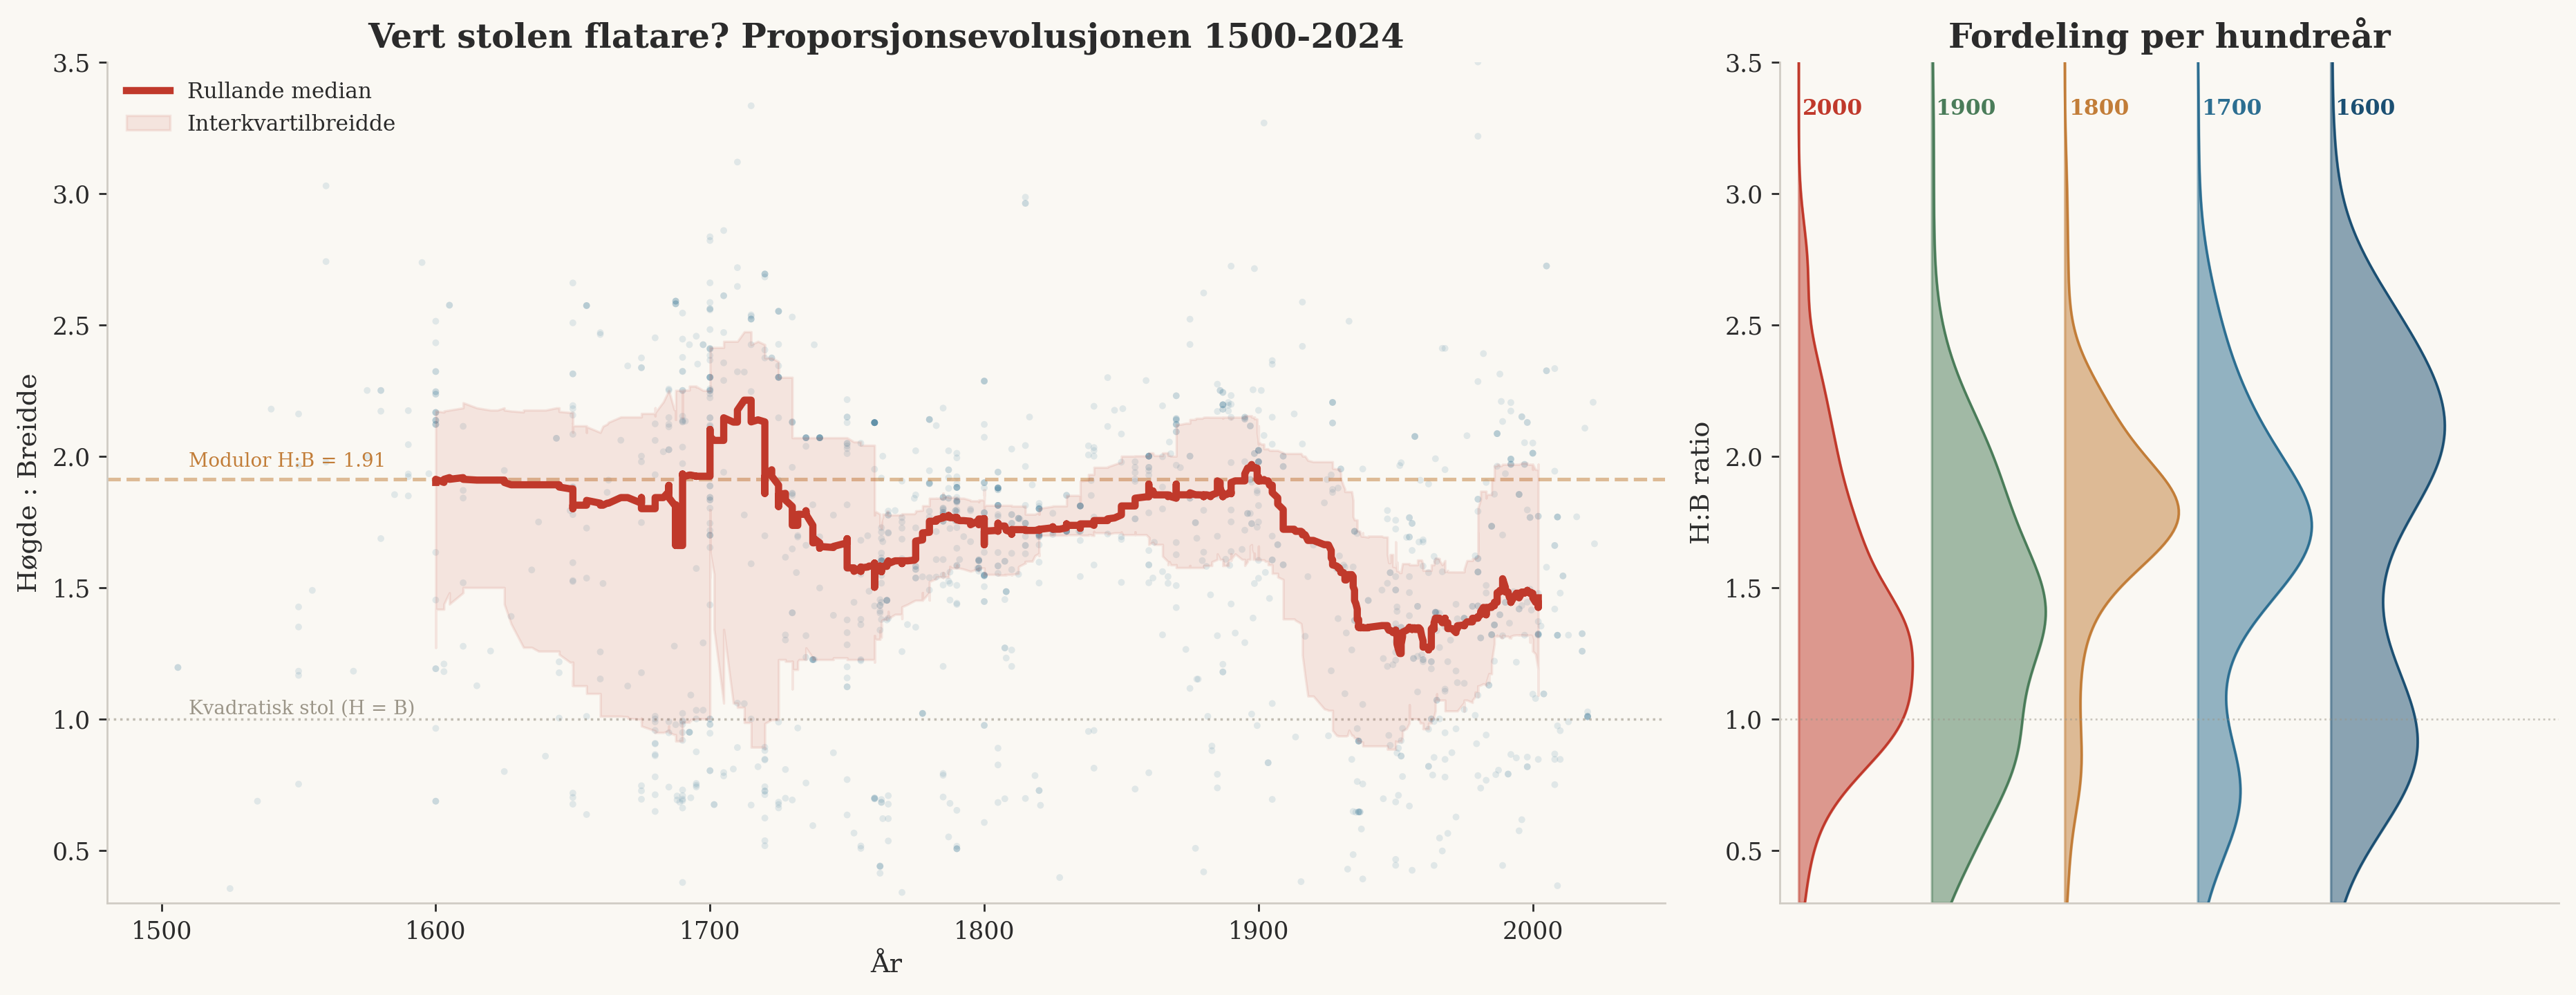
\includegraphics[width=\columnwidth]{01_squatness_index.png}
  \caption{Proporsjonsdrift: $H/W$-ratio per hundreaar. Gullsnittet ($\varphi = 1{,}618$) er markert. Modernismen bryt drastisk med tradisjonen.}
  \label{fig:hw_ratio}
\end{figure}

$H/W$-ratioen driftar nedover frå 1,68 (1600-talet) til 1,37 (2000-talet). Gullsnittet, som mange designteoretikarar har tillagt normativ kraft, vert \emph{passert} ein gong på veg nedover, ikkje \emph{stabilisert rundt}. Det er ikkje ein attraktor; det er ein stasjon toget passerer. Spreiinga ($\sigma$) aukar på 1900-talet til over 1,0, noko som tyder at modernismen ikkje berre skapte nye proporsjonar, men \emph{sprengde det tidlegare proporsjonsbandet}.


\subsection{NMK og V\&A: to produksjonsgeografiar}

\begin{table}[H]
\centering
\caption{Gjennomsnittleg stolhøgde per museum per hundreår.}
\label{tab:nmk_va}
\begin{tabular}{@{}lrrrr@{}}
\toprule
\textbf{Hundreår} & \textbf{$N_{\text{NMK}}$} & \textbf{$\bar{H}_{\text{NMK}}$} & \textbf{$N_{\text{V\&A}}$} & \textbf{$\bar{H}_{\text{V\&A}}$} \\
\midrule
1600-talet &  59 & 111,1 & 199 &  86,5 \\
1700-talet & 196 & 102,2 & 385 &  80,3 \\
1800-talet & 182 &  86,5 & 282 &  89,3 \\
1900-talet & 179 &  88,5 & 458 &  74,1 \\
2000-talet &  44 &  77,7 &  37 &  67,7 \\
\bottomrule
\end{tabular}
\end{table}

\begin{figure}[H]
  \centering
  
\includegraphics[width=\columnwidth]{fig9_nmk_va_hogde.pdf}
  \caption{Norske vs. britiske stolar: gjennomsnittleg hogde per hundreaar. NMK-stolar er systematisk hogare i tidlege periodar.}
  \label{fig:nmk_va}
\end{figure}

Tre funn stikk seg ut:

\begin{enumerate}
  \item \textbf{NMK-stolane er systematisk høgare.} I 1600-talets gjennomsnitt er nordiske stolar 24,6 cm høgare enn britiske. Dette reflekterer ein distinkt \emph{nordisk stoltradisjon}: høge ryggar, kraftige konstruksjonar, gjerne barokkstolar med stolperammer og utskorne dekorasjonar i lokal eik og ask.

  \item \textbf{Konvergens på 1800-talet.} Høgdeskilnaden fell til berre $-$2,8 cm i 1800-talets gjennomsnitt: nordiske og britiske stolar har vorte nær identiske i ein sentral dimensjon. Industrialiseringa, masseproduksjonen og den internasjonale utstillingskulturen (Verdsustillingane frå 1851 og frametter) har drive formkonvergens på tvers av geografi.

  \item \textbf{Divergens igjen etter 1900.} På 1900-talet er NMK-stolane igjen 14,4 cm høgare. Den skandinaviske modernismen (Aalto, Jacobsen, Mogensen, Korsmo) skapte ein \emph{regional identitet} innanfor det moderne prosjektet: ein skandinavisk stol er i snitt ein annleis stol enn ein britisk.
\end{enumerate}

Mønsteret er ikkje monoton konvergens, men \emph{oscillerande drift}: divergens, konvergens, ny divergens. Geografi forsvinn ikkje som formkraft; han vert midlertidig overskugga av industrialisering og kjem tilbake i ny form.


\subsection{Vektreduksjon: materialeffektivitet over tid}

\begin{table}[H]
\centering
\caption{Estimert vekt (kg) per hundreår. Berre stolar med vektestimat ($n = 150$).}
\label{tab:weight}
\begin{tabular}{@{}lrrrr@{}}
\toprule
\textbf{Hundreår} & \textbf{$N$} & \textbf{$\bar{W}$ (kg)} & \textbf{Median (kg)} & \textbf{$\sigma$} \\
\midrule
1600-talet &  13 & 19,4 & 18,7 & 13,0 \\
1700-talet &  50 & 20,8 & 20,4 &  7,9 \\
1800-talet &  41 & 16,2 & 13,9 & 14,4 \\
1900-talet &  32 & 25,1 & 14,4 & 26,1 \\
2000-talet &  14 & 11,9 &  6,8 & 14,9 \\
\bottomrule
\end{tabular}
\end{table}

Medianvekta fell frå 20,4 kg (1700-talet) til 6,8 kg (2000-talet): ein reduksjon på 67\,\%. Denne vektreduksjonen speglar overgangen frå massive trekonstruksjonar til tynne stålprofil, laminerte skjel og sprøytestøypt plast. Som Artikkel I viste, er materialpaletten vorte meir kompleks (stigande $H'$), men materiala vert brukte meir \emph{effektivt}: meir form per kilogram.

\begin{quote}
\textbf{Materialeffektivitet:} Dersom me definerer materialeffektivitet som forholdet mellom funksjonelt overflatareal og masse, aukar denne effektiviteten dramatisk over tid. Ein barokkstol frå 1700-talet brukar 20 kg for å halde eitt menneske; ein plastkrakk frå 2020 brukar 3 kg for same funksjon. Materiala har vorte \emph{smartare}: dei ber meir med mindre.
\end{quote}

\begin{figure}[H]
  \centering
  \includegraphics[width=\columnwidth]{01_weight_over_time.png}
  \caption{Vektreduksjon over tid: medianvekt per hundreaar. Fraa massive barokkstolar til minimale plastkrakkar.}
  \label{fig:weight}
\end{figure}

Ekstremverdiane illustrerer spennvidda: den lettaste stolen i databasen er ein plastkrakk av Giorgio Decurso frå 1972 (0,4 kg, polypropylen); den tyngste er ein sofa av John Henry Belter frå 1856 (103 kg, eik og palisander). Ein faktor på 257 i vekt under same funksjon. Denne eine statistikken falsifiserer funksjonsdeterminismen meir effektivt enn noko anna funn: dersom form (og vekt) følgde funksjon, ville denne ratioen vere nær 1,0.

\subsubsection{Vekt per materiale}

Vektdata er tilgjengelege for 150 stolar, nok til å identifisere materialspesifikke mønster:

\begin{table}[H]
\centering
\caption{Estimert medianvekt per hovudmateriale.}
\label{tab:weight_mat}
\begin{tabular}{@{}lrrr@{}}
\toprule
\textbf{Materiale} & \textbf{$n$} & \textbf{Median (kg)} & \textbf{Gj.snitt (kg)} \\
\midrule
Plast & 7 & 8,2 & 8,7 \\
Mahogni & 23 & 13,3 & 13,3 \\
Furu & 30 & 14,8 & 15,6 \\
Bjørk & 40 & 16,3 & 17,4 \\
Bøk & 34 & 18,9 & 21,8 \\
Eik & 21 & 14,1 & 24,5 \\
Stål & 11 & 13,0 & 25,4 \\
Kryssfiner & 16 & 24,6 & 33,8 \\
\bottomrule
\end{tabular}
\end{table}

Plastkrakken er lettast (median 8,2 kg), medan kryssfiner er overraskande tung (24,6 kg), truleg fordi kryssfiner-stolar ofte er store, polstra konstruksjonar (Eames Lounge Chair-typen). Materialet dikterer ikkje berre proporsjonen, men òg massen.


\subsection{Stilperiodar: emergente merkelappar}

\begin{figure}[H]
  \centering
  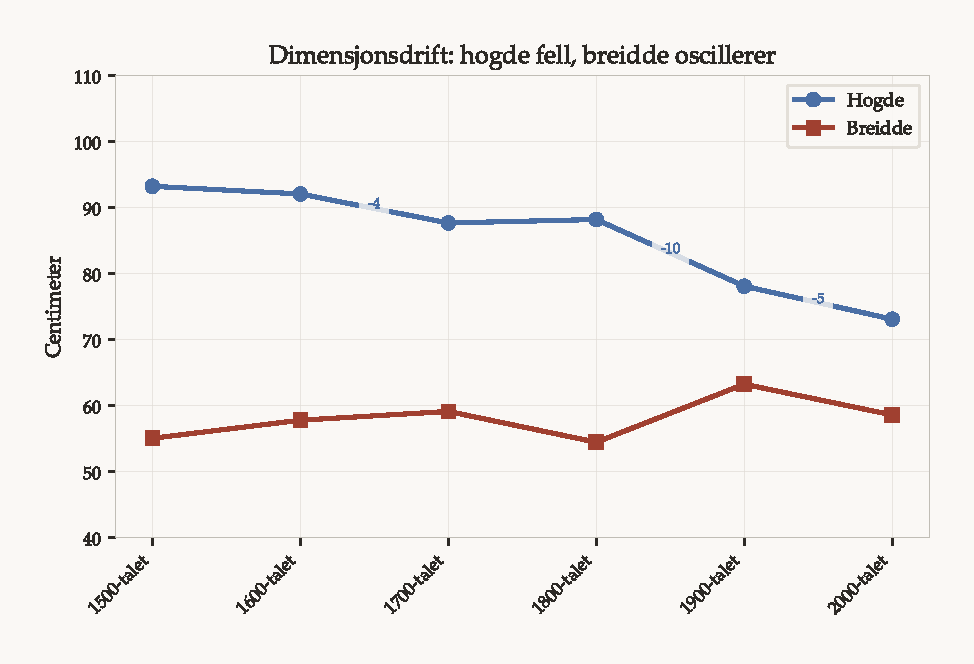
\includegraphics[width=\columnwidth]{fig14_dimensjonsdrift.pdf}
  \caption{Dimensjonsdrift: gjennomsnittleg hogde fell, medan breidde oscillerer. Hogda fell mest mellom 1800- og 1900-talet.}
  \label{fig:drift}
\end{figure}

\subsection{Nasjonale materialfingeravtrykk: chi-kvadrattest}

Ein $\chi^2$-test på materialdistribusjon per nasjonalitet gjev $\chi^2 = 633{,}8$ ($p < 10^{-100}$, $\text{df} = 45$). Kvar nasjon etterlét eit distinkt materielt fingeravtrykk (figur~\ref{fig:chi2}).

\begin{figure}[H]
  \centering
  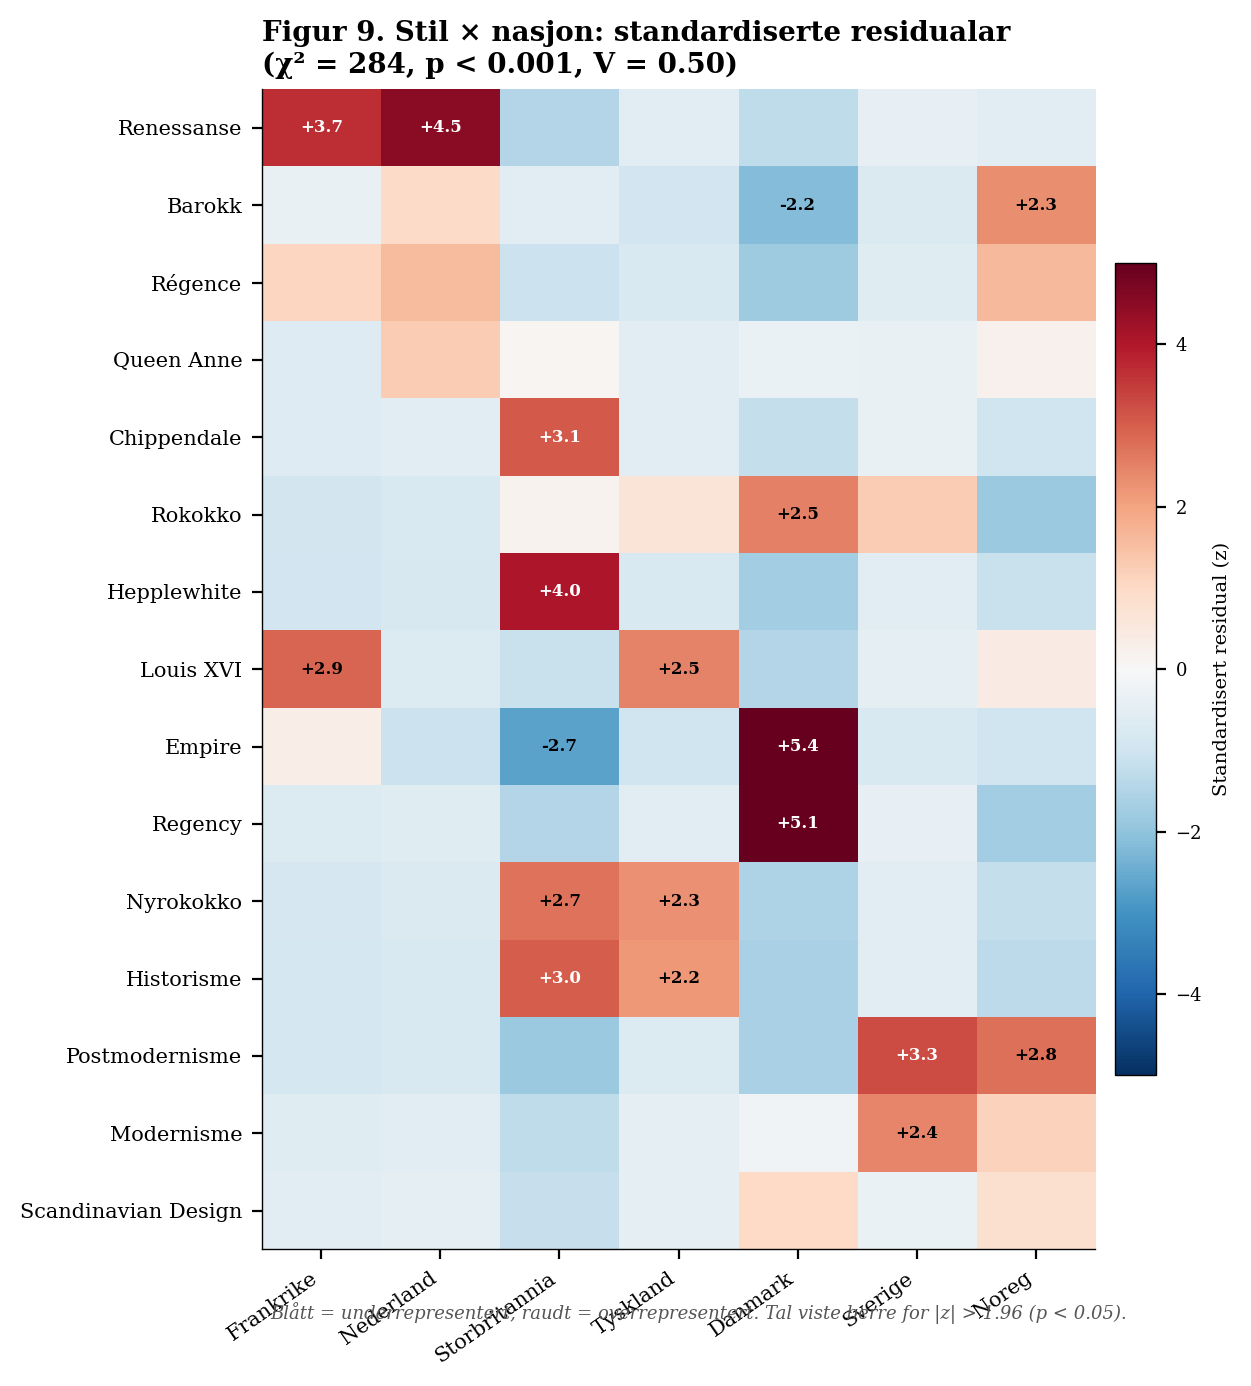
\includegraphics[width=\columnwidth]{fig9_chi2_residualar.png}
  \caption{Nasjonale materialfingeravtrykk. Standardiserte $\chi^2$-residualar. Raude celler = overrepresentasjon; blaae = underrepresentasjon. Noreg: bjork $+10{,}8\sigma$, furu $+8{,}2\sigma$. Storbritannia: mahogni $+4{,}3\sigma$.}
  \label{fig:chi2}
\end{figure}

Dei sterkaste assosiasjonane er:
\begin{itemize}
  \item \textbf{Noreg}: bjørk ($+10{,}8\sigma$), furu ($+8{,}2\sigma$), kryssfiner ($+3{,}8\sigma$). Norske stolar er laga av det som veks i norske skogar.
  \item \textbf{Storbritannia}: mahogni ($+4{,}3\sigma$). Det koloniale treet er det britiske fingeravtrykket.
  \item \textbf{Italia}: nøttetre ($+9{,}4\sigma$). Renessansens og barokkens favorittmateriale.
  \item \textbf{Danmark}: kryssfiner ($+5{,}8\sigma$), stål ($+3{,}6\sigma$). Den danske modernismens signaturmaterialar.
  \item \textbf{Tyskland}: stål ($+4{,}6\sigma$). Bauhaus og den industrielle tradisjonen.
\end{itemize}

Desse fingeravtrykka er ikkje tilfeldige; dei reflekterer djupe materialøkologiar. Noreg har bjørkeskog; Storbritannia har koloniar med mahogni; Italia har nøttetrekultur; Danmark og Tyskland har industriell infrastruktur for stål og kryssfiner.

Nasjonale \textbf{H/W-profilar} kvantifiserer denne dimensjonen: Noreg har $H/W = 1{,}91$ (hogast og smalast), Finland $H/W = 1{,}10$ (flatast og breiast), Storbritannia 1,32, Frankrike 1,23. Noreg og Finland er ytterpunkta i det nordiske formrommet: Noreg si barokk-arv gjev hoege ryggar; Finland si Aalto-arv gjev flate, breie profil. Materialøkologien (bjørk vs. bjørk!) er den same, men designkulturen er diametralt ulik. Dette stadfestar at materiale ikkje \emph{determinerer} form; det \emph{avgrensar} formrommet, men innanfor det rommet er det kulturelle val som vel posisjon.

\textbf{Materiell entropi per nasjon} stadfestar dette mønsteret. Storbritannia har den høgaste materialentropien ($H' = 4{,}72$ bits, $S = 66$ materialar), noko som reflekterer imperiet sin tilgang til globale ressursar. Finland har den lågaste ($H' = 3{,}33$ bits, $S = 18$): Aalto-effekten har skapt eit nasjonalt bjørkemonopol som minner om mahogni-monopolet i NMK, men drive av lokal materialideologi snarare enn kolonial import.

\subsection{Stilmigrasjon: retensjon og assimilering}

Stilperiodar migrerer ulikt mellom nasjonar. Me kan identifisere to ytterpunkt:

\begin{itemize}
  \item \textbf{Retinerte stilar}: stilar som er sterkt knytte til éin nasjon. Barokk er retinert i Noreg (90\,\% av barokkstolane med nasjonalitetsdata er norske). Hepplewhite og Chippendale er retinerte i Storbritannia.
  \item \textbf{Migrerte stilar}: stilar som spreier seg jamt. Funksjonalisme er den mest migrerte stilen: berre 39\,\% norsk, resten fordelt mellom fleire nasjonar. Empire er delt 50/50 mellom Noreg og Danmark.
\end{itemize}

Retensjon korrelerer med materialøkologi: barokk i Noreg er assosiert med lokale treslag (eik, bjørk), medan funksjonalisme brukar globale materialar (stål, kryssfiner) som er tilgjengelege uavhengig av geografi. Materialtilgangen avgjer ikkje berre forma, men òg kor langt ein stil kan reise.

\subsection{Dimensjonsdrift}

\begin{figure}[H]
  \centering
  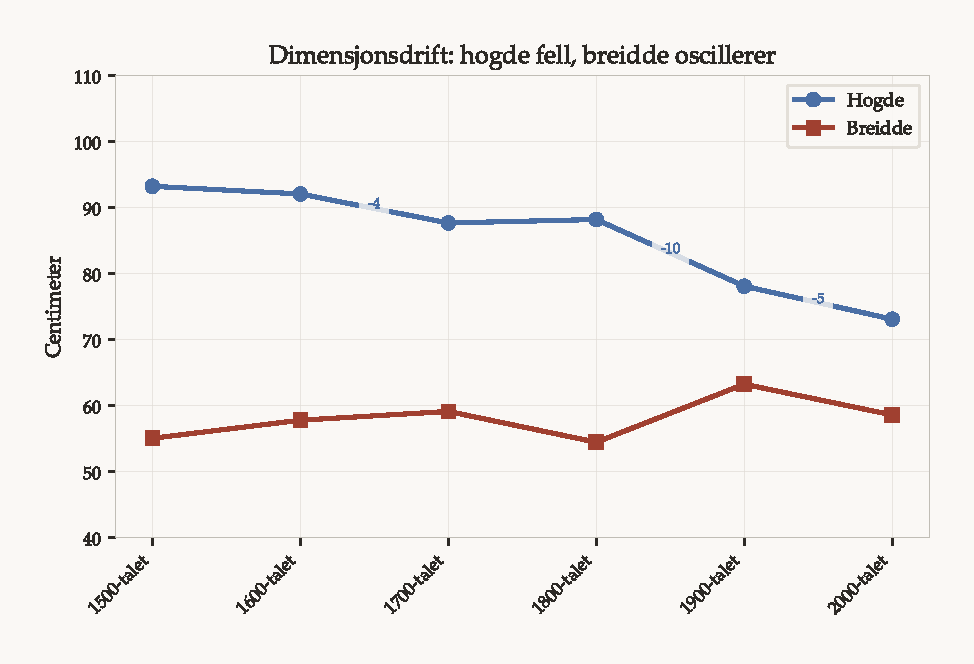
\includegraphics[width=\columnwidth]{fig14_dimensjonsdrift.pdf}
  \caption{Dimensjonsdrift: gjennomsnittleg hogde fell, medan breidde er meir stabil. Den storste drifta fell saman med industrialiseringa (1800--1900).}
  \label{fig:drift}
\end{figure}

Den dimensjonelle drifta mellom hundreår er ikkje jamn. Me reknar ein forenkla avstandsmetrikk i standardavvik-einingar: den storste drifta fell mellom 1800- og 1900-talet (0,314 SD), som korresponderer med industrialiseringa. Stolen vert lågare ($\Delta H = -10$ cm) og breiare ($\Delta W = +9$ cm) i dette intervallet. Industrialiseringa er det sterkaste geometriske sjokket i heile tidsserien.

\subsection{Affordanse-matrisa: materialet avgjer teknikken}

Kryssanalyse av materiale og teknikk avdekkjer ein tydeleg \textbf{affordanse-matrise}: kvart materiale ``tillèt'' berre visse teknikkar, og stengjer andre ute. Mahogni og eik tillèt tapping (22\,\% og 21\,\%) og skjering (14\,\% og 17\,\%), men ikkje sveising. Stål tillèt sveising (11\,\%) og formbøying (23\,\%), men ikkje tapping eller skjering. Plast er det mest fleksible: skruing (32\,\%), formbøying (25\,\%) og polstring (32\,\%). Kvart materiale opnar visse regionar av formrommet og stengjer andre. Materialet er ikkje ein nøytral berar av form; det er ein \emph{aktiv formgjevande kraft}.

\subsection{Stilperiodar: emergente merkelappar}

Berre 22,9\,\% av stolane ($n = 524$) har stilmerke. Blant desse dominerer barokk ($n = 92$), historisme ($n = 64$), funksjonalisme ($n = 47$), empire ($n = 36$) og postmodernisme ($n = 27$). 12 nasjonalitetar er representerte, der Storbritannia dominerer (57,6\,\%) grunna V\&A-samlinga sitt tyngdepunkt.

Stilperiodane er ujamt fordelte og overlappande i tid. Dei er ikkje diskrete kategoriar med skarpe grenser, men \emph{emergente klynger} i formrommet. Artikkel III vil demonstrere kvantitativt at stilmerket er den svakaste prediktoren for ein stol sin faktiske geometri.


% ================================================================
\section{Diskusjon}

\subsection{Mot konvergens eller divergens?}

Funksjonalismen predikerer konvergens: dersom form følgjer funksjon, og funksjonen er konstant, burde formvariasjonen minke over tid. Variasjonskoeffisienten burde falle monotont. Data syner det motsette: CV oscillerer og viser ikkje ein klar nedovertrend. Formvariasjonen er ikkje driven primært av funksjonell optimering, men av skiftande seleksjonstrykk: nye materialar, nye produksjonsteknologiar, nye kulturelle preferansar.

\subsection{Norske stolar er signifikant hogare}

Ein Mann-Whitney U-test stadfestar at norske stolar (median = 95 cm, $n = 153$) er signifikant hogare enn britiske (median = 89 cm, $n = 766$): $p = 3{,}3 \times 10^{-10}$, Cohen's $d = 0{,}70$ (stor effektstorleik). Skilnaden på 17,7 cm er ikkje tilfeldig; han reflekterer ulike materialøkologiar.

\subsection{Materialet predikerer dimensjonar}

Mann-Whitney U-testar syner at materialet har ein direkte, statistisk signifikant effekt på hogde: stål-stolar er 13 cm lågare enn andre ($p < 10^{-10}$), plast-stolar 14 cm lågare ($p < 10^{-7}$), medan mahogni-stolar er 6 cm \emph{hogare} ($p = 0{,}002$). ANOVA stadfestar dette: treslag predikerer hogde signifikant ($F = 4{,}5$, $p = 0{,}002$) og breidde ($F = 3{,}3$, $p = 0{,}015$). Interessant nok er effekten på \emph{djupn} ikkje-signifikant ($F = 2{,}1$, $p = 0{,}087$), noko som tyder at djupn er den mest funksjonsdeterminerte dimensjonen: uansett materiale treng stolen ein viss djupn for å romme ein sitjande kropp.

\subsection{Korrelasjonsstruktur: hogde er uavhengig av breidde}

Pearson-korrelasjonsmatrisa avdekkjer ein overraskande struktur: $r(H,W) = 0{,}04$ ($p = 0{,}08$), altso \emph{ikkje signifikant}. Hogde og breidde er statistisk uavhengige. Derimot er $r(W,D) = 0{,}52$ ($p < 10^{-128}$): breidde og djupn er sterkt korrelerte. Setet (W og D) er ein sameint konstruksjon; ryggen (H) er ein uavhengig variabel. Stolen er \emph{ikkje} eitt samla objekt; han er to objekt: eit sete og ein rygg, med ulike determinantar.

\subsection{Djupn: den funksjonsdeterminerte dimensjonen}

Eit nøkkelfunn er at \textbf{djupn} har konsekvent lågast variasjonskoeffisient av dei tre hovuddimensjonane: $\text{CV}_D = 0{,}18$--$0{,}31$ mot $\text{CV}_H = 0{,}26$--$0{,}38$ og $\text{CV}_W = 0{,}14$--$0{,}47$. ANOVA stadfestar dette: materialeffekten på djupn er ikkje-signifikant ($F = 2{,}1$, $p = 0{,}087$), i motsetnad til hogde ($p = 0{,}002$) og breidde ($p = 0{,}015$). Djupn er den einaste dimensjonen som faktisk vert avgrensa av kroppen: eit sete treng ein viss djupn for å romme lara, uansett materiale. Dette er det narmaste me kjem ``form follows function'' i heile datasettet: eitt spor av funksjonell determinisme i eit hav av materiell og kulturell variasjon.

Samstundes konvergerer $W/D$-ratioen mot 1,0 over tid: fraa 1,27 (1500-talet) til 1,01 (2000-talet). Setet vert perfekt kvadratisk. Modernismens stol har eit sete som er like breitt som det er djupt.

\subsection{Kompaktheit: materialeffektivitet kvantifisert}

Me definerer \textbf{kompaktheit} som omsluttande volum per kilogram ($V/W$, i cm$^3$/kg). Denne ratioen stig fraa 14\,757 cm$^3$/kg (1700-talet) til 38\,445 cm$^3$/kg (2000-talet): ein auke paa 2,6 gonger. Moderne materialar gjev meir form per kilo. Ein plastkrakk okkuperer same rom som ein barokkstol, men veg ein fjerdedel. Materialeffektiviteten er den kvantitative manifestasjonen av overgangen fraa ``tunge'' til ``smarte'' materialar.

\subsection{Hogdekurva: fraa rygg til krakk og tilbake}

Høgda per tiaar avdekkjer ein dramatisk narrativ. Fraa 95 cm (1700-talet) fell gjennomsnittleg hogde monotont til eit botnpunkt paa \textbf{64 cm i 1970}: modernismen har redusert stolen til nesten ein krakk. Men sa kjem ein braa reversering: paa 1980-talet stig hogda tilbake til \textbf{85 cm} (+19 cm paa eitt tiaar). Postmodernismen henta ryggen tilbake. Denne oscillasjonen er eit direkte eksempel paa exploration/exploitation-dynamikken: modernismen utforskar den rygglause stolen; postmodernismen returnerer til ryggen som eit estetisk og funksjonelt val.

Forholdet mellom setehøgde og totalhøgde (SH/H) stadfestar dette: frå 52\,\% på 1600-talet til 72\,\% på 1900-talet og 98\,\% på 2000-talet. Stolen er bokstavleg talt i ferd med å miste ryggen. Barokkstolen har ein rygg som utgjer nesten halvparten av den totale høgda; den moderne stolen er nesten berre sete. Denne overgangen reflekterer ikkje ergonomisk optimering (ryggar er framleis nyttige), men ein \emph{materiell og kulturell} endring: nye materialar mogeleggjer sjølvberande konstruksjonar, og modernismens estetikk favoriserer minimale profil.

\subsection{Designarprofil: kvar navigator si posisjon}

Databasen inneheld stolar av kanoniske designarar som okkuperer radikalt ulike posisjonar i formrommet:

\begin{table}[H]
\centering
\caption{Designarprofil: dimensjonar og materialar for namngjevne designarar.}
\label{tab:designers}
\begin{tabular}{@{}lrrrlll@{}}
\toprule
\textbf{Designar} & \textbf{$n$} & \textbf{$\bar{H}$} & \textbf{$H/W$} & \textbf{Hovudmateriale} & \textbf{Periode} \\
\midrule
Chippendale & 11 & 99,7 & 1,53 & Mahogni (73\,\%) & 1755--1850 \\
Thonet & 12 & 73,2 & 1,58 & Bøk, rotting & 1836--1925 \\
Aalto & 18 & 60,5 & 1,37 & Bjørk (100\,\%) & 1929--1954 \\
Jacobsen & 7 & 60,8 & 1,22 & Kryssfiner, stål & 1955--1967 \\
Eames & 18 & 51,6 & \textbf{0,93} & Stål, glasfiber & 1945--2007 \\
Wegner & 4 & 49,2 & \textbf{0,83} & Bøk, lær & 1944--1970 \\
\bottomrule
\end{tabular}
\end{table}

To observasjonar er slåande. For det fyrste: \textbf{Eames og Wegner har $H/W < 1{,}0$}: stolane deira er \emph{breiare enn dei er høge}. Stolen har vorte eit horisontalt objekt. For det andre: Chippendale sin $H/W = 1{,}53$ og Thonet sin $H/W = 1{,}58$ er nær gullsnittet ($\varphi = 1{,}618$), medan Eames og Wegner har brote fullstendig med denne tradisjonen. Materialvalet forklarer overgangen: mahogni og bøk (vertikale, stolpebaserte konstruksjonar) gjev høge proporsjonar; stål og glasfiber (sjølvberande skjel) gjev låge, breie profil.

Kvar designar er ein \emph{navigator} som har funne ein distinkt posisjon i tilpassingslandskapet. Posisjonene er ikkje tilfeldige; dei er determinerte av materialet sin affordanse.

\subsection{Kvifor Modulor sviktar}

Le Corbusier sin prediksjon feilar ikkje fordi han misrekna kroppsdimensjonar, men fordi han antok at kroppen sin geometri åleine bestemmer stolen sin geometri. Empirisk er den gjennomsnittlege stolen 25--40 cm kortare enn prediksjonen i kvar epoke. Denne systematiske skilnaden reflekterer det \citet{pye1968} kalla \textbf{arbeidets natur}: den materielle praksisen der handverkar og materiale forhandlar om den endelege forma. Treverk dikterer andre proporsjonar enn stål; skjering dikterer andre enn sveising. Modulor ignorerer materialet sin stemme.

\subsection{Formrom-trajektorie: stolens vandring gjennom 500 aar}

Me kan følgje stolens vandring gjennom formrommet ved å plotte sentroiden (gjennomsnittleg $H$, $W$, $D$) per hundreaar. Trajektoria avdekkjer ein systematisk drift:

\begin{itemize}
  \item 1500-talet: $H = 92{,}8$ cm, $W = 54{,}4$ cm, $H/W = 1{,}71$. Høg, smal. Renessansestolen.
  \item 1700-talet: $H = 88{,}1$ cm, $W = 59{,}6$ cm, $H/W = 1{,}48$. Litt breiare, litt lågare.
  \item 1900-talet: $H = 78{,}2$ cm, $W = 62{,}5$ cm, $H/W = 1{,}25$. Dramatisk lågare og breiare.
  \item 2000-talet: $H = 79{,}5$ cm, $W = 62{,}6$ cm, $H/W = 1{,}27$. Stabilisert.
\end{itemize}

Sentroiden driftar frå det øvre venstre hjørnet av $H/W$-rommet (høg, smal) mot det nedre høgre (låg, brei). Denne drifta er den geometriske manifestasjonen av det me har observert i materialdata: overgangen frå massive stolperammer i lokalt tre til slanke industrielle konstruksjonar.

\subsection{Signaturstolar: den mest typiske stolen per epoke}

For kvar epoke kan me identifisere den \emph{signaturstolen}: stolen som ligg nærmast sentroiden i det tredimensjonale formrommet ($H \times W \times D$). Desse stolane er ikkje nødvendigvis dei mest berømte, men dei mest \emph{representative}:

\begin{itemize}
  \item \textbf{1700-talet}: ein anonym armstol i mahogni, messing og tekstil ($H = 88$, $W = 58$, $D = 52$ cm). Avstand frå sentroiden: berre 2,2 cm. Kolonialtida sin generiske stol.
  \item \textbf{1900-talet}: OK-2002-0155, ein stol i metall, plast og stål ($H = 79$, $W = 63$, $D = 62$ cm). Avstand: 1,1 cm. Industrialderen sin generiske stol.
  \item \textbf{2000-talet}: 360 Chair i aluminium, polyuretan og stål ($H = 78$, $W = 63$, $D = 63$ cm). Avstand: 2,9 cm.
\end{itemize}

Signaturstolen har gått frå mahogni til plast, frå handverk til industri, frå kolonialt tre til petrokjemisk polymer. Men dimensjonane har konvergert: signaturstolen frå 1900 og 2000 er nesten identiske i storleik. Det som har endra seg, er \emph{materialet}, ikkje forma.

\subsection{Geografi som formkraft}

Det mest overraskande funnet er den oscillerande divergens-konvergens-divergens-syklusen mellom NMK og V\&A. Geografi er ikkje ein historisk levning som vert vaska vekk av globaliseringa: det er ein aktiv, periodisk formkraft som vekslar mellom å dominere og å vike. Den nordiske stoltradisjonens gjenkomst i skandinavisk modernisme syner at lokale materialøkologiar og handverkstradisjonar kan reinskrivast i nye teknologiske regime.

Denne oscillerande dynamikken svarar til det \citet{eldredge1972} kalla \textbf{punctuated equilibrium}: lange periodar med stabilitet avbrote av raske endringsperiodar. Industrialiseringa er eit slikt ``brot'' som midlertidig homogeniserer form, men nye lokale optima oppstår raskt i det nye landskapet.

\subsection{Stolen vert lettare og lågare}

Kombinasjonen av fallande høgde og fallande vekt er ikkje tilfeldig. Nye materialar (stål, kryssfiner, plast) mogeleggjer slankare profil og tynne tverrsnitt. Ein stol treng ikkje lenger vere 20 kg for å bere ein menneskekropp; 5 kg held. Denne materialeffektiviteten frigjer formrommet: designaren er ikkje lenger avgrensa av trevirket sin stivheit, men kan utforske geometriar som tidlegare var fysisk umoglege. Formrommet utvidar seg irreversibelt.

\subsection{Avgrensingar}

Tre atterhald er naudsynte. For det fyrste er dimensjonsdata heterogene i kvalitet: museumskuratorar måler stolar på ulike vis, og nokre verdiar (særleg volum) har store uteliggjarar. For det andre dominerer V\&A datasettet ($n = 1\,613$ av 2\,284), noko som gjev ein britisk bias. For det tredje er vektestimata berre tilgjengelege for 150 stolar (6,6\,\% av utvalet), noko som gjer vektanalysen indikativ snarare enn statistisk robust.


% ================================================================
\section{Konklusjon}

Produksjonsgeografien skriv seg inn i stolen sin form på tre vis. For det fyrste er den gjennomsnittlege stolen vorte lågare og djupare over tid, ikkje fordi kroppen har endra seg, men fordi materialteknologien og den kulturelle konteksten har det. For det andre er høgdeskilnaden mellom nordiske og britiske stolar eit direkte mål på geografien sin formkraft, ein kraft som oscillerer mellom konvergens og divergens. For det tredje syner den systematiske underprediksjonen av Modulor at stolens geometri ikkje kan deduserast frå kroppen åleine.

Form følgjer ikkje funksjon. Form driftar i eit landskap der geografi, materiale, teknologi og tid alle utøver seleksjonstrykk. Den neste artikkelen vil demonstrere at dimensjonar og materialkombinasjonar kan \emph{predikere} stilperiode med høg presisjon, samstundes som stilmerket sjølv er den svakaste prediktoren for faktisk geometri.


% ================================================================
\bibliographystyle{plainnat}
\bibliography{references}

\end{document}
